\documentclass{article}

\usepackage[french]{babel}
\usepackage[utf8]{inputenc}
\usepackage{amsmath}
\usepackage{graphicx} %package to manage images
\graphicspath{ {./images/} }

%%%%%%%%%%%%%%%% Lengths %%%%%%%%%%%%%%%%
\setlength{\textwidth}{15.5cm}
\setlength{\evensidemargin}{0.5cm}
\setlength{\oddsidemargin}{0.5cm}

%%%%%%%%%%%%%%%% Variables %%%%%%%%%%%%%%%%
\def\projet{2}
\def\titre{Méthode du gradient conjugué / Application à l’équation de la chaleur}
\def\groupe{4}
\def\equipe{12468}
\def\responsible{Enzo Médina}
\def\secretary{Perig Herau}
\def\others{Ghofrane Hamdouni, Hector Piteau}

\begin{document}

%%%%%%%%%%%%%%%% Header %%%%%%%%%%%%%%%%
\noindent\begin{minipage}{0.98\textwidth}
  \vskip 0mm
  \noindent
  { \begin{tabular}{p{7.5cm}}
      {\bfseries \sffamily
        Projet \projet} \\ 
      {\itshape \titre}
    \end{tabular}}
  \hfill 
  \fbox{\begin{tabular}{l}
      {~\hfill \bfseries \sffamily Groupe \groupe\ - Equipe \equipe
        \hfill~} \\[2mm] 
      Responsable : \responsible \\
      Secrétaire : \secretary \\
      Codeurs : \others
    \end{tabular}}
  \vskip 4mm ~

  ~~~\parbox{0.95\textwidth}{\small \textit{Résumé~: Dans ce projet nous cherchons à implémenter des algorithmes, direct et itératifs, de résolution de systèmes linéaires Ax = b avec A de grande taille. Nous allons nous intéresser tout particulièrement aux systèmes linéaires symétriques définis positifs et creux et discuter des efficacités et complexités de ces algorithmes.  } \sffamily  }
  \vskip 1mm ~
\end{minipage}

%%%%%%%%%%%%%%%% Main part %%%%%%%%%%%%%%%%
\section*{Présentation du travail réalisé}
    Dans la suite de ce rapport, nous allons vous présenter le travail que nous avons réalisé au cours du projet. Puis nous conclurons avec un retour sur le gain d'expérience que nous a apporté ce projet. 
\subsection*{Décomposition de Cholesky} 
    Cette partie a pour objectif d'écrire une méthode de factorisation en utilisant la décomposition de Cholesky classique, puis incomplète. \\
    
    1) Dans un premier temps, on s'occupe de la décomposition classique. Étant donné qu'on parcourt chaque élément de la matrice ($O(n^{2})$) et que les éléments diagonaux nécessitent d'accéder à l'ensemble des éléments de la ligne ($O(n)$), l'algorithme possède une complexité cubique $O(n^{3})$. \\
    \iffalse
    Elle est définie par la formule suivante : 
    \begin{align}
        t_{i,i}^2 &= a_{i,i} - \sum_{k=1}^{i-1} t_{i,k}^2 \\
        t_{i,i}^2 &= \frac{a_{i,i} - \sum_{k=1}^{i-1} {t_{i,k}*t_{j,k}}}{t_{i,i}} \quad j \ge i\quad
    \end{align}
    \fi
    
    2) En utilisant l'algorithme dense, le coût total en temps est cubique ($O(n^3)$) car on effectue un parcours sur une ligne (compléxité linéaire) pour chaque élément de la matrice (au nombre d'éléments quadratique). \\

\iffalse
\begin{itemize}
    \item N : Ce paramètre nous permet de connaître le nombre d'éléments extra diagonaux non nuls souhaités. Étant donné que la matrice retournée est symétrique, on considère uniquement le côté supérieur (ou inférieur) de la matrice pour la valeur de N. Ainsi, on a $0 <= N <= n*(n-1)/2$ avec n la taille de la matrice. \\
    
    \item Size : Paramètre permettant de définir la taille souhaitée de la matrice retournée. On a besoin d'un seul paramètre car on retourne une matrice carrée. Très utile pour les différents tests. \\
\end{itemize}
\fi
    
    3) On souhaite retourner une matrice symétrique. Pour cela, on utilise le fait que le produit d'une matrice et de sa transposée retourne une matrice symétrique ($A = B . ^tB$ implique A symétrique), et on lui assigne une diagonale dominante pour obtenir le caractère définie positive. Les termes extra diagonaux sont eux assignés aléatoirement par la fonction \textit{randint}, puis un certain nombre sont assignés à 0 aléatoirement de même. \\
    
  4) La factorisation incomplète de Cholesky est très similaire à la factorisation classique. Il suffit simplement de vérifier si on a des éléments nuls dans la matrice d'origine, auquel cas on retourne 0 à la même position pour la matrice générée. \\
  
  Nous avons essayé plusieurs tests de performances :
  \begin{enumerate}
      \item Une génération de 1000 matrices de petites tailles (3 et 4). \\
      Les temps d'exécution des factorisations classiques et incomplètes sont très similaires (au centième de seconde près).
      Dans le cas de matrices contenant uniquement des 0 dans les éléments diagonaux, on remarque que la factorisation incomplète est à peine meilleure. A l'inverse, dans le cas de matrices sans termes nuls, c'est la factorisation classique qui plus performante, ce qui est logique car on rajoute un test dans la version incomplète. \\
      
      \item Une unique matrice de très grande taille (700 x 700) \\
      Avec une matrice entièrement rempli d'éléments extra diagonaux nuls, le résultat est sans appel : \textbf{27s de temps d'exécution par la factorisation classique contre 0.2s pour la factorisation incomplète}.
      En revanche, pour des matrices ne contenant pas de 0, elles restent équivalentes.
  \end{enumerate}
  
  On comprends alors tout l'intérêt de chercher à réduire les matrices pour obtenir un maximum d'éléments extra diagonaux nuls. Les calculs sont bien plus rapides (Dans le cas de notre matrice 700 * 700, on parle d'une méthode 100 fois meilleure). \\
  
5) On définit une fonction pour obtenir le conditionnement du produit \(^tT^{-1} . T^{-1}\) et le conditionnement classique de A. Les résultats sont très proches (précision \(10^{-8}\)). Cependant, on remarque que pour la moitié des tests, le conditionnement calculé est supérieur au conditionnement de A. C'est donc un mauvais préconditionneur. L'autre moitié du temps, il est donc inférieur et correspond à un bon préconditionneur.


    
\subsection*{Méthode du gradient conjugué}
\paragraph{}
    Dans cette partie nous avons implémenté l'algorithme itératif de la méthode du gradient conjugué, dont le pseudo-algorithme est donné sur la page Wikipedia de l'algorithme \cite{gradconjugwiki}.

\paragraph{}
    Tout d'abord, il nous a été donné dans le sujet une implémentation Matlab dans laquelle nous avons relevé certains non respect d'un standard de programmation sain. Parmi ces derniers, nous avons relevé que les noms des variables ne sont pas toujours explicites, ce qui freine la compréhension de l'algorithme. De plus, le seuil de précision constituant la condition d'arrêt est inscrit en dur dans l'algorithme. Il est donc impossible de le changer au cours de l'exécution.
    
\paragraph{}
    Cet algorithme est cependant différent de la méthode de Cholesky décrite précédemment, car il ne nécessite pas d'utiliser un algorithme comme celui de Gauss (seules les remontées sont à effectuer). Ainsi, on obtient une complexité quadratique au lieu de cubique la plupart du temps. Cependant, dans le cas de matrices spécifiques, le gain de complexité est négligeable puisque la décomposition de Cholesky trouve directement la bonne forme de matrice pour simplifier la suite.

\paragraph{}
    La première méthode est est une implémentation directe. La présence de multiples produits matriciels de complexités respectivement linéaire et quadratiques, dans une boucle qui s'arrête à une précision demandée, donnent à l'algorithme une complexité en $O(log(i)*n^2)$ avec i la précision souhaitée. Deux paramètres ont été ajoutés, pour avoir un contrôle manuel sur la précision et le nombre maximum d'itérations directement en entrée de l'algorithme. 
    
\paragraph{}
    La seconde méthode utilise un préconditionneur sur la matrice d'entrée, dans le but de réduire le nombre d'itérations de l'algorithme. Cette méthode est de complexité similaire, mais produit moins d'itérations (bien que temporellement, elle soit plus coûteuse à l'exécution à cause du nombre de transformations), comme on peut le voir dans la figure \ref{fig:conj_precond}. 
    
\begin{figure}[ht]
    \centering
    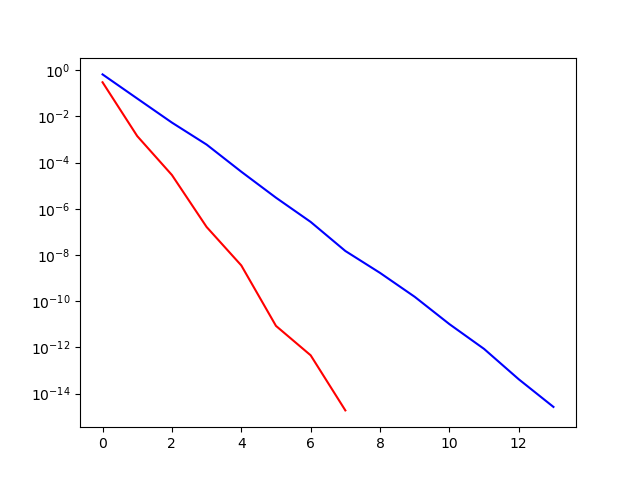
\includegraphics[width=0.7\columnwidth]{conjgrad_comp.png}
    \caption{Comparaison du nombre d'itérations des algorithmes du gradient conjugué, avec (rouge) et sans (bleu) préconditionneur, avec des matrices de taille 100.}
    \label{fig:conj_precond}
\end{figure}

\paragraph{}
    Pour éviter l'utilisation d'inversions de matrices (souvent imprécises et propices à nombre d'erreurs), une double remontée gaussienne a été utilisée, en utilisant la décomposition du préconditionneur en un produit de deux matrices triangulaires symétriques. Ainsi, une fonction pour automatiser ces remontées (sur une matrice triangulaire supérieure ou inférieure) a été définie.
    
    
\subsection*{Application à l’équation de la chaleur}
    Cette partie a pour but de mettre en oeuvre les deux précédente parties 
    afin de résoudre une équation aux dérivées partielles, l'équation de la chaleur. 
    Le but étant de simuler l'évolution de la température sur une grille de points. Pour cela, nous allons commencer par présenter la méthode des différences finies : 
    \paragraph{} 
    Les méthodes des différences finie est une technique de recherche de solutions 
    approchées d’équations aux dérivées partielles qui consiste à résoudre un
    système de relations (schéma numérique) liant les valeurs des fonctions 
    inconnues en certains points suffisamment proches les uns des autres. 
   \begin{enumerate}
   	\item { Approximation des dérivées }
   	\paragraph{}
   
 	Pour la dérivée seconde par rapport au sous-jacent $ x_{\i}$ au point $ x_{\i}$ 
   en utilisant une approximation centrée basée sur la formule de Taylor  on aura alors : 
   	
   $	$$\frac{\partial^2 t}{\partial x^2}$$  = $$\frac{t( xj + dx , yj ) - 2*t( xj , yj ) + t( xj-dx , yj)}{(dx)^2 }$$ $ 
   
   \paragraph{}
   	En remplaçant les termes de l'équation %add reference de l'equation de la chaleur 
   	on aura après simplification du calcul :
   	
   	$t ( i , j ) = 4 *b(i , j ) * h^2 - t(i+1 , j) - t(i-1 , j)-t(i , j+1)-t(i , j-1))$ 
   	
   	les indices des coefficients varient entre [ i-1 , i+1 ] et [ j-1 , j+1] 
   	ce qui induit nécessairement l'utilisation des blocs tridiagonales . En effet  , 
   	soit j $\in$ [0 , N] fixe :
   	\paragraph{}
   	
   	$t(j,1) = a*t(j+1 , 1) + b*t(j+1,1) + c*t(j+1,0)$, et en généralisant :
   	\paragraph{}
   	\iffalse
    $t(j,2) = a*t(j+1 , 2) + b*t(j+1,2) + c*t(j+1,1)$
    \paragraph{}
    $t(j,3) = a*t(j+1 , 3) + b*t(j+1,3) + c*t(j+1,2)$ 
    \paragraph{}
    .
    \paragraph{} 
    .
    \paragraph{}
   	\fi
   $t(j,n-1) = a*t(j+1 , n-1) + b*t(j+1,n-1) + c*t(j+1,n-2)$ 
   
   \paragraph{} 
   Ce qui explique que le problème peut s'exprimer sous la forme d'un 
   système linéaire $Ax=b$ où la matrice A est une matrice tridiagonale par blocs 
   de taille $N^2$x$N^2$ avec chaque diagonale est remplie respectivement par a , b , c ( dans ce cas 1 , -4 , 1 )  
   \paragraph{}
   \item{implémentation python} 
 	\paragraph{} 
 	Pour pouvoir appliquer les méthodes du gradient conjugué pour la résolution il 
   faut commencer par introduire les matrices A , B et T . 
 	\begin{enumerate}
 		\item { La Matrice A est une matrice tridiagonale par blocs . 
     En partant d'une matrice diagonale en utilisant la bibliothèque numpy, 
     on ajoute une autre matrice diagonale supérieure d'ordre 1 et sa transposée 
     puis on annule des termes pour avoir des blocs diagonaux.
 		\textbf{ la transposée n'est pas une opération linéaire } 
 		Pour la construction de A, l'algorithme est de complexité O( $N^4)$ } 

 		\item{La Matrice B se déduit du second membre de l'équation . 
 		Pour la construction de B, l'algorithme est de complexité O( $N^2)$   } 
   	\item { Résolution pour un radiateur au centre (figure \ref{centre}) }  
   	\begin{figure}[h]
   	\centering
   		\begin{minipage}[c]{\linewidth}
   			\centering
   			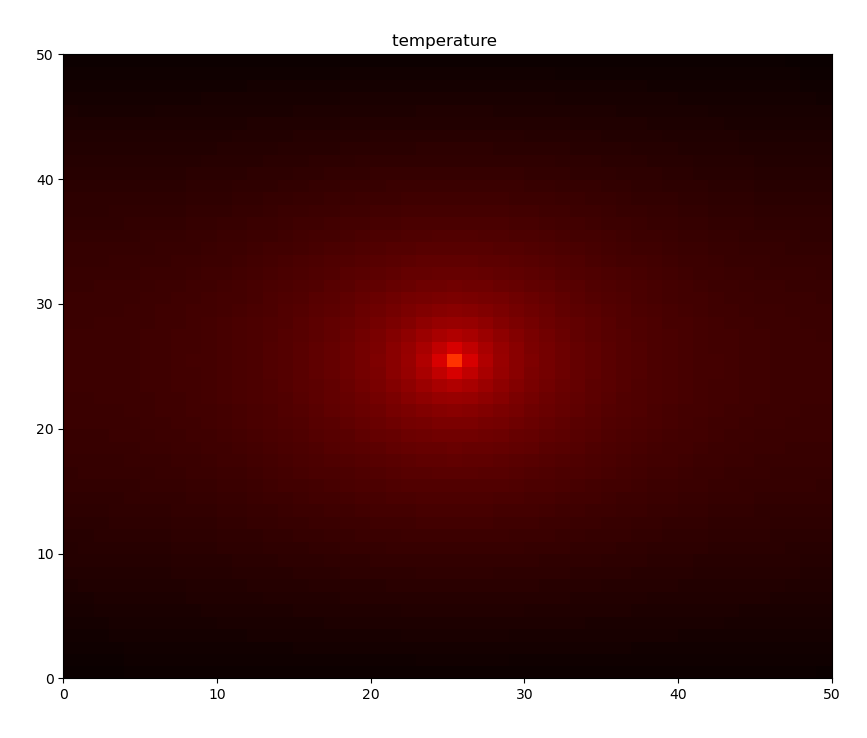
\includegraphics[width=3cm,height=3cm]{centreN50T5.png}
   			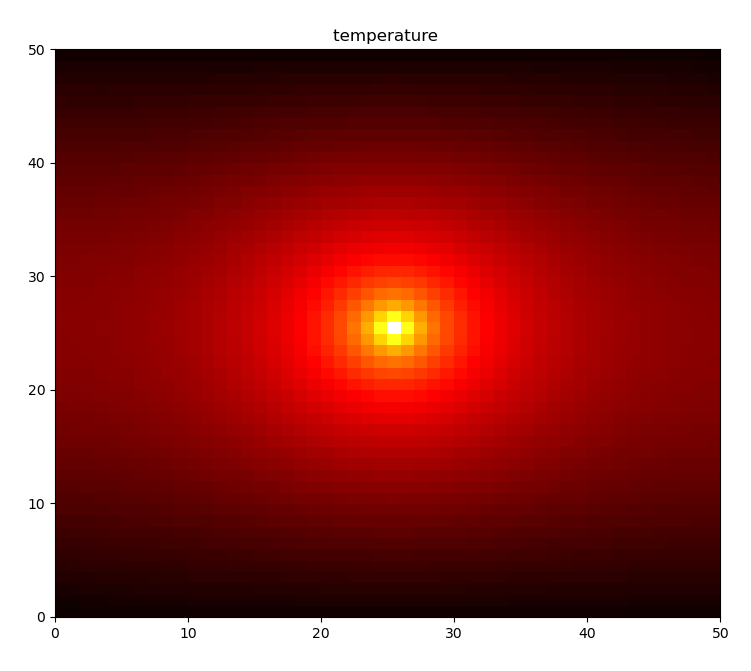
\includegraphics[width=3cm,height=3cm]{centreN50T25.png}
   			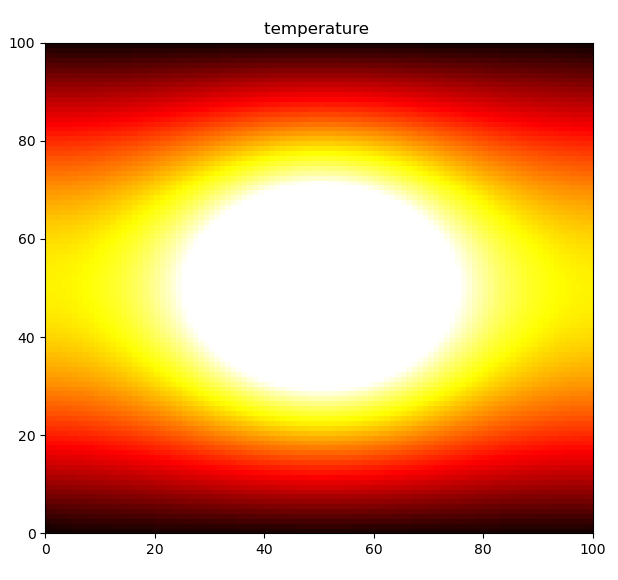
\includegraphics[width=3cm,height=3cm]{centreN100T25.png}
   			\caption{Illustrations pour les couples (N,T) : (50,5), (50,25), (100,25) }
   			\label{centre}
   	\end{minipage} \hfill 
\end{figure} 

\paragraph{Commentaires } 
On voit bien que le résultat est cohérent pour un même N  . 
A une même température pour N=100 la température est plus élevée au centre que pour N=50 . 
Ce qui explique que pour des grandes valeurs de N , la résolution est plus précise puisque elle se fait en tout point de l'espace .  
   	\item{Résolution pour un radiateur mis au nord (figure \ref{nord})} 
   	\begin{figure}[h]
   	\centering
   		\begin{minipage}[c]{.46\linewidth}
   			\centering
   			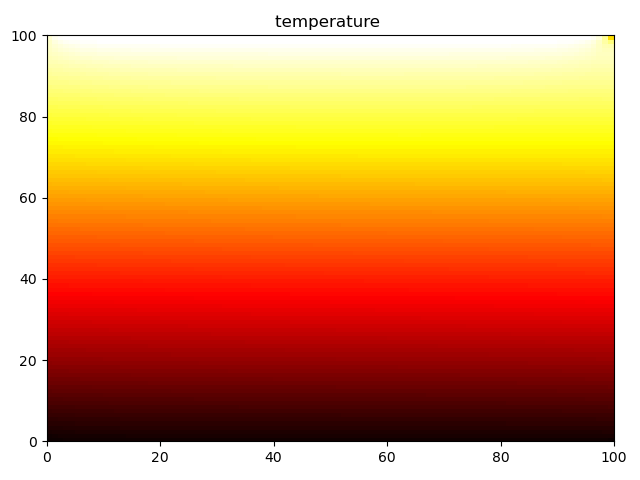
\includegraphics[width=3cm,height=3cm]{coteN100T5.png}
   			\caption{Illustration pour N=100 T=5° }
   			\label{radiateur sur le cote ( N=100 ,T=5°)}
   		\end{minipage}
   		\label{nord}
\end{figure} 
\paragraph{Commentaires} 
On voit bien que le résultat est cohérent pour un même N  . 
\paragraph{}
A une même température pour N=100 la température est plus élevée au centre que pour N=50 . 
Ce qui explique que pour des grandes valeurs de N , la résolution est plus précise puisque elle se fait en tout point de l'espace . 



\item{Commentaires sur les deux cas d'illustration } 
\begin{itemize}

\item {Dans les deux cas de la mise en place du radiateur , la différence situe essentiellement à la modification de la matrice du second membre qui est le B . }
\item{ Pour une valeur de N suffisamment grande  , dans l'une des mises en place du radiateur , pour une valeur faible de T( valeur du second membre de l'équation ) , la résolution est moins précise . En effet , prenant l'exemple le produit d'une ligne L1 (1 , $N^2$ ) et d'une colonne C1  ( $N^2$ , 1 ) pour vérifier l'égalité : $ L1*C1 = 5 $ 
	\paragraph{} 
la multiplication entre les termes et l'addition des valeurs proches  augmentent les erreurs }

\end{itemize}
  
   \end{enumerate}
   
   
   
   
   
   \paragraph{}
    Une telle résolution est couteuse en temps : Le temps d'exécution du programme est proportionnel à la valeur de $N^2$x$N^2$. Or Python est à typage dynamique et est interprété et non compilé ce qui fait qu'il est 'lent'. 
   \iffalse
   % --------------------------------------------------------------------------------
    \item{Pour aller plus loin  } 
   \paragraph{}
   Une équation de la forme  : 
   \paragraph{}
   $A $$\frac{\partial^2 t}{\partial x^2}$$ + B	$$\frac{\partial^2 t}{\partial x^2 \partial y^2}$$ + C 	$$\frac{\partial^2 t}{\partial y^2}$$ +G = 0 $ 
  \paragraph{}
   Avec dans ce cas B est nulle et elliptique puisque $ B - 4 xAC < 0 $ 
   Cela signifie que l’on calcule un champ U : il faut calculer la valeur de U en tout
   point de l’espace. 
   La dépendances des termes en( i , j) ( i-1 , j) ( i+1 , j) ( i , j+1 ) et ( i , j-1) 
   induit des décalages lignes et colonnes. 
   \paragraph{}
   Mais pour décaler les colonnes Le seul moyen est d’utiliser la transposée : 
   Décaler d’une colonne : décaler les lignes de la transposée et prendre la
   transposé du résultat
  
   \textbf{PROBLEME!! }
   \paragraph{}  
   La transposition de matrice n’est pas une opération linéaire
   \paragraph{}
   Une équation du type : $A X + B X.T = C $ n’est pas une opération linéaire.
   Donc on ne peut pas écrire simplement ce problème sous la forme d’une Simple multiplication de matrices. 
   On peut s’en sortir en écrivant un système de $N^2$ équations à $N^2$ inconnus. 
   Ce qui illustre bien la méthode utilisée dans cette partie. 
   \textbf{On voit donc que les équations elliptiques sont très coûteuses en mémoire et
   en calcul} 
  \item { Introduction aux approches spectrales } 
  \paragraph{}
  En se limitant à des opérations mathématiques qu'on appelle convolution la base des transformées de Fourier  : 
  \paragraph{}
  Soient $T*= TF(T), Lap*=TF(lap) , f*=TF (f)$ 
  \paragraph{}
  où TF signifie "transformée de fourrier"
  \paragraph{}
  $T*xLap*= f$
  \paragraph{}
  $T*= \frac{f*}{Lap*}$ 
  \paragraph{}
  $T = TF-1 (\frac{f*}{Lap*})$  
  \textbf{ AVANTAGE : l’algorithme FFT est très rapide (en Nlog(N) )} 
  
  Les approches spectrales, qui passent par une Transformée de Fourier, sont souvent les plus
  rapides (grâce à l’algorithme FFT). 
  
  % --------------------------------------------------------------------------------
   \fi
   
   \end{enumerate} 

   
  
   
    

%%%%%%%%%%%%%%%% End part %%%%%%%%%%%%%%%%
\section*{Conclusion et apports du projet}
\paragraph{}
    Les deux méthodes et leur amélioration respective (décomposition de Cholesky
    incomplète et gradient conjugué avec préconditionneur) sont viables dans le 
    cas de la résolution d'un système linéaire en un temps raisonnable. 
    Cependant, la seconde méthode semble faire ses preuves pour un apport non 
    négligeable en complexité en nombre d'itérations, et ainsi peut être appliquée 
    à des simulations comme celle de la troisième partie du projet.

\begin{thebibliography}{9}
\bibitem{gradconjugwiki} 
Algorithme de la décomposition de Cholesky sur Wikipedia.
\\\texttt{https://en.wikipedia.org/wiki/Conjugate\_gradient\_method}
\end{thebibliography}


\end{document}
